% !TeX program = xelatex
% !TeX encoding = utf8
% !TeX root = RegT1E_HS22.tex

%% TODO: publish to CTAN
\documentclass[margin=normal]{tex/hsrzf}

%%%%%%%%%%%%%%%%%%%%%%%%%%%%%%%%%%%%%%%%%%%%%%%%%%%
% Packages
\usepackage{multicol}
\usepackage[export]{adjustbox}
\usepackage{bm}
\usepackage{color, colortbl}
\usepackage{trfsigns}
\usepackage{graphicx}
\usepackage{tabularx}
\usepackage{mathrsfs}
\usepackage{tikz}
\usepackage{xcolor}
\usepackage{hyperref}

\usetikzlibrary{plotmarks}

\usepackage{pgfplots}
\usepackage{lscape}


\usetikzlibrary{plotmarks}

\definecolor{TabularBackgroundColor}{rgb}{0.83,0.96,0.96}
\definecolor{TabularTitleColor}{rgb}{0.89,0.94,0.94}
\definecolor{RefColor}{rgb}{0.59,0.88,0.72}

\newcommand{\skript}[1]{{\scriptsize \color{RefColor}Skript S.#1}}
\newcommand{\tiltewithref}[2]{\texorpdfstring{#1 {\scriptsize \color{RefColor}Skript S.#2}}{#1}}
%% TODO: publish to CTAN
\usepackage{tex/hsrstud}

%% Language configuration
\usepackage{polyglossia}

\setdefaultlanguage[variant=swiss]{german}

%% License configuration
\usepackage[
    type={CC},
    modifier={by-nc-sa},
    version={4.0},
    lang={german},
]{doclicense}


%%%%%%%%%%%%%%%%%%%%%%%%%%%%%%%%%%%%%%%%%%%%%%%%%%%
% Metadata

\course{Elektrotechnik}
\module{RegT1E}
\semester{Herbstsemester 2022}

\authoremail{joel.leirer@ost.ch}
\author{\textsl{Joël Leirer} -- \texttt{\theauthoremail}}

% did someone help you with this work?
\contributors{
  % do not forget to add yourself!
}

\title{\texttt{\themodule} Zusammenfassung}
\date{\thesemester}

%%%%%%%%%%%%%%%%%%%%%%%%%%%%%%%%%%%%%%%%%%%%%%%%%%%
% Document

\begin{document}

% use roman numberals for introductiory pages
\pagenumbering{roman}

\maketitle


% show the names of the people who contributed to this document.
% \section*{Contributors}
% \thecontributors

\section*{Lizenz}
\doclicenseThis

\clearpage
\tableofcontents

% actual content
\clearpage
\setcounter{page}{1}
\pagenumbering{arabic}
\section{Allgemeines}
\subsection{Begriffe}
\small
\begin{itemize}
      \item Prozess
            \begin{itemize}
                  \item Die Gesamtheit zusammenwirkender Vorgänge, welche durch
                        die Materie, Energie und Information
                        umgefort, transportiert und gespeichert wird.
            \end{itemize}

      \item System
            \begin{itemize}
                  \item Ist gegenüber der Umwelt abgegrenzt, hat Eingänge,
                        Ausgänge (und Zustand).
                  \item (LTI-/)LZI-Systeme: Lineare-ZeitInvariante Systeme
                        (Linearität gilt, System ist unabhängig von zeitlicher Verschiebung
                        --> DGL mit Konst. Koeff.)
            \end{itemize}

      \item Modell
            \begin{itemize}
                  \item Beschreibung von Systemen, wird genutzt für
                        Erklärung, Prognose, Gestaltung und Optimierung.
                  \item Es gibt kein "richtiges Modell",
                        ein Modell beschreibt ein System nur so genau wie nötig.
            \end{itemize}
      \item Modellieren
            \begin{itemize}
                  \item Teilsysteme erstellen und diese
                        in weitere Teilsysteme aufzutrennen.
                        So erhält man einfache Grundsysteme (Grundglieder),
                        welche sich einfach Mathematisch beschreiben lassen.
                        Zusätzlich kehern einige Teilsysteme in ihrer
                        Struktur oft wieder und können wiederverwendet werden.

                  \item Top-Down: System in Teilsysteme teilen
                  \item Bottom-Up: System aus Grundglieder aufbauen
            \end{itemize}
      \item Grundglieder
            \begin{itemize}
                  \item Kleinste Teilsysteme. Sie können weiter augeteilt werden, siehe Abschnitt Grundglieder
            \end{itemize}
      \item Sprungantwort
            \begin{itemize}
                  \item Reaktion des Systems auf die Sprungfunktion. Siehe LTI-Systeme

            \end{itemize}
      \item Schrittantwort
      \item \begin{itemize}
                  \item Reaktion des Systems auf die Schrittfunktion. Siehe LTI-Systeme
            \end{itemize}
      \item Ausgleich
            \begin{itemize}
                  \item Prozesse ohne Ausgleich: Sprungantwort wächst Grenzenlos an
                  \item Prozess mit Ausgleich: Sprungantwort strebt endlichem Wert zu
            \end{itemize}
\end{itemize}
\normalsize

\subsection{Regelkreis}
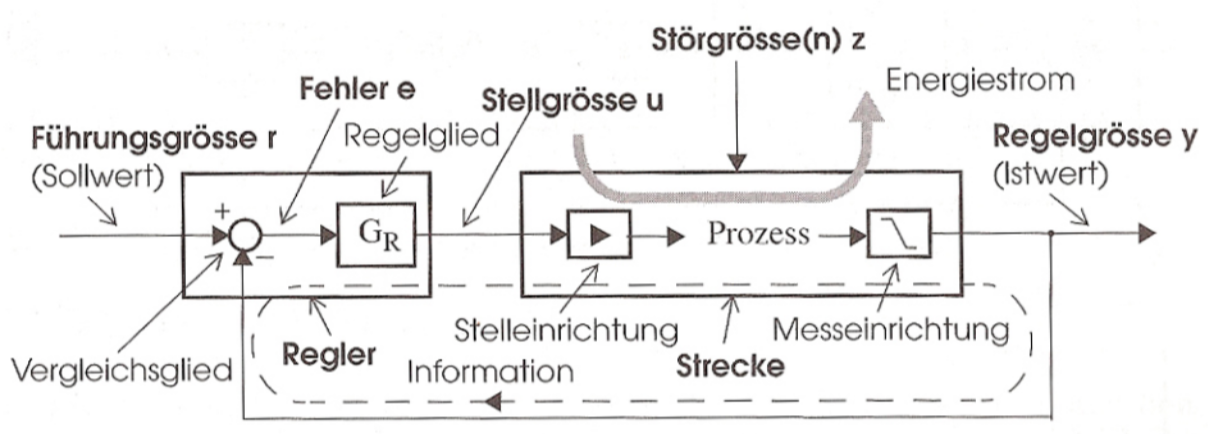
\includegraphics{img/Regelkreis.png}

\subsection{Steuern und Regeln}
\begin{minipage}{0.5\textwidth}
      \subsubsection*{Steuerung}

\end{minipage}%
\begin{minipage}{0.5\textwidth}
    a  
\end{minipage}


%%%%%%%%%%%%%%%%%%%%%%%%%%%%%%%%%%%%%%%%%%%
%Packages
%Needs Commands:
%\newcommand{\skript}[1]{{\scriptsize \color{RefColor}Skript S.#1}}
%\newcommand{\titlewithref}[2]{\texorpdfstring{#1 {\scriptsize \color{RefColor}Skript S.#2}}{#1}}
%
%%%%%%%%%%%%%%%%%%%%%%%%%%%%%%%%%%%%%%%%%%%
%Content
%%%%%%%%%%%%%%%%%%%%%%%%%%%%%%%%%%%%%%%%%%%

\begin{landscape}
    \subsection{\titlewithref{Grundglieder}{26,29,30,31,193,202}}
    \begingroup
    \scriptsize
    \newcommand{\ImageWidth}{70pt}
    \begin{tabularx}{\linewidth}{|p{100pt}|p{160pt}|p{60pt}|p{80pt}|p{120pt}|p{80pt}|}
          \hline
          \textbf{Benennung}
           &
          \textbf{Funktion}
           &
          \textbf{UTF\textsuperscript{1}}
           &
          \textbf{Symbol}
           &
          \textbf{Sprungantwort}
           &
          \textbf{Plot}
          \\
          \hline
          \hline
          %%%%%%%%%%%%%%%%%%%%%%%%%%%%%%%%%%%%%%%%%%%%%%%%%%%%%%%%%%%%%%%%%%%%%%%%%%%%%%%%%%%%%%%%%%%%%
          \textbf{P-Glied\textsuperscript{2}}
          \newline Proportionalglied
           &
          $y = K \cdot u$
           &
          $K$
           &
          \raisebox{-.5\height}{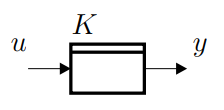
\includegraphics[width = \ImageWidth]{img/DIN-Symbole/Proportionalglied.png}}
           &
          $K$
           &
          \raisebox{-.5\height}{
                \resizebox{\ImageWidth}{!}{%
                      \begin{tikzpicture}
                            % Grid
                            \draw[help lines,dashed] (0,0) grid (5,3);

                            % Axes
                            \draw[very thick,latex-latex] (0,3.25) node[left]{$y(t)$}
                            |- (5.25,0) node[below]{$t$};

                            % Plot function
                            \draw[ultra thick,teal] (-0.5,0) node[left,black](s0){$0$}
                            -- ++(0.5,0)
                            plot[domain=0:5,
                                        samples = 50,
                                        smooth]({\x}, {2});
                      \end{tikzpicture}
                }
          }
          \\
          \hline
          \rowcolor{TabularBackgroundColor}
          %%%%%%%%%%%%%%%%%%%%%%%%%%%%%%%%%%%%%%%%%%%%%%%%%%%%%%%%%%%%%%%%%%%%%%%%%%%%%%%%%%%%%%%%%%%%%
          \textbf{I-Glied}
          \newline(Idealer Integrierer)
           &
          $y(t) = K \cdot \int \limits _{t=0} ^{t} u(\tau) d\tau + y(0)$
          \newline $\dot{y}(t) = K \cdot u(t)$
           &
          $K \frac{1}{s}$
           &
          \raisebox{-.5\height}{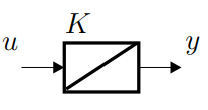
\includegraphics[width = \ImageWidth]{img/DIN-Symbole/Integrator.png}}

           &
          $K \cdot t$
           &
          \raisebox{-.5\height}{
                \resizebox{\ImageWidth}{!}{%
                      \begin{tikzpicture}
                            % Grid
                            \draw[help lines,dashed] (0,0) grid (5,3);

                            % Axes
                            \draw[very thick,latex-latex] (0,3.25) node[left]{$y(t)$}
                            |- (5.25,0) node[below]{$t$};

                            % Plot function
                            \draw[ultra thick,teal] (-0.5,0) node[left,black](s0){$0$}
                            -- ++(0.5,0)
                            plot[domain=0:5,
                                        samples = 50,
                                        smooth]({\x},);
                      \end{tikzpicture}
                }
          }
          \\
          \hline
          %%%%%%%%%%%%%%%%%%%%%%%%%%%%%%%%%%%%%%%%%%%%%%%%%%%%%%%%%%%%%%%%%%%%%%%%%%%%%%%%%%%%%%%%%%%%%
          \textbf{Totzeit-Glied}
           &
          $y(t) = u(t-T_t)$
           &
          $e^{-s T_t}$
           &
          \raisebox{-.5\height}{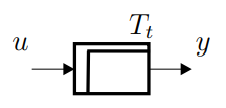
\includegraphics[width = \ImageWidth]{img/DIN-Symbole/Totzeitglied.png}}
           &
          $\sigma(t-T) = \begin{cases}
                                     0, t<T     \\
                                     1, t\geq T \\
                               \end{cases}$
           &
          \raisebox{-.5\height}{
                \resizebox{\ImageWidth}{!}{%
                      \begin{tikzpicture}
                            % Grid
                            \draw[help lines,dashed] (0,0) grid (5,3);

                            % Axes
                            \draw[very thick,latex-latex] (0,3.25) node[left]{$y(t)$}
                            |- (5.25,0) node[below]{$t$};

                            % Plot function
                            \draw[ultra thick,teal] (-0.5,0) node[left,black](s0){$0$}
                            -- ++(0.5,0)
                            plot[domain=0:5,
                                        samples = 100,
                                  ]({\x},{ (\x<=2) * 0  + (\x>2) * 2});
                      \end{tikzpicture}
                }
          }
          \\
          \hline
          \rowcolor{TabularBackgroundColor}
%%%%%%%%%%%%%%%%%%%%%%%%%%%%%%%%%%%%%%%%%%%%%%%%%%%%%%%%%%%%%%%%%%%%%%%%%%%%%%%%%%%%%%%%%%%%%
          \textbf{D-Glied}
          \newline Idealer Differenzierer
           &
          $y(t) = K \cdot \frac{du(t)}{dt} = K\cdot \dot{u}(t)$
           &
          $K \cdot S $
           &
          \raisebox{-.5\height}{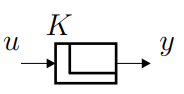
\includegraphics[width = \ImageWidth]{img/DIN-Symbole/D-Glied.png}}
           &
          $K\cdot \delta(t)$
           &
          \raisebox{-.5\height}{
                \resizebox{\ImageWidth}{!}{%
                      \begin{tikzpicture}
                            % Grid
                            \draw[help lines,dashed] (0,0) grid (5,3);

                            % Axes
                            \draw[very thick,latex-latex] (0,3.25) node[left]{$y(t)$}
                            |- (5.25,0) node[below]{$t$};

                            % Plot function
                            \draw[ultra thick ,teal] (2,0) -- node[left]{$\delta$} (2,2);
                            
                      \end{tikzpicture}
                }
          }
          \\
          \hline
          %%%%%%%%%%%%%%%%%%%%%%%%%%%%%%%%%%%%%%%%%%%%%%%%%%%%%%%%%%%%%%%%%%%%%%%%%%%%%%%%%%%%%%%%%%%%%
          \textbf{DT\textsubscript{1}-Glied}
          {
                \tiny 
                \newline Realisierbarer Differenzierer
                \newline K: Verstärkung
                \newline T: Zeitkonstante
          }
           &
          $ y(t) + T \cdot \dot{y}(t) = K \dot{u}(t)$
          \newline $y(t) = K \dot{u}(t) - T \cdot \dot{y}(t)$
          
           &
          $\frac{K \cdot s}{1+T_s}$
           &
          \raisebox{-.5\height}{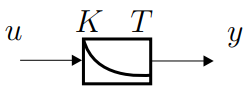
\includegraphics[width = \ImageWidth]{img/DIN-Symbole/DT-Glied.png}}
           &
          $\frac{K}{T}\cdot e^{-\frac{t}{T}}$
           &
          \raisebox{-.5\height}{
                \resizebox{\ImageWidth}{!}{%
                      \begin{tikzpicture}
                            % Grid
                            \draw[help lines,dashed] (0,0) grid (5,3);

                            % Axes
                            \draw[very thick,latex-latex] (0,3.25) node[left]{$y(t)$}
                            |- (5.25,0) node[below]{$t$};

                            % Plot function
                            \draw[ultra thick,teal] (-0.5,0) node[left,black](s0){$0$}
                            -- ++(0.5,0)
                            plot[domain=0:5,
                                        samples = 50,
                                        smooth]({\x},{2.5*exp(-(\x))});
                      \end{tikzpicture}
                }
          }
          \\
          \hline   
          \rowcolor{TabularBackgroundColor}
          %%%%%%%%%%%%%%%%%%%%%%%%%%%%%%%%%%%%%%%%%%%%%%%%%%%%%%%%%%%%%%%%%%%%%%%%%%%%%%%%%%%%%%%%%%%%%
          \textbf{PT\textsubscript{1}-Glied}
          {
                \tiny \newline K: Verstärkung
                \newline T: Zeitkonstante
          }
           &
          $ T\dot{y} + y = K u(t)$
          \newline $T= \frac{1}{K_I \cdot K_P} $
          \newline $K = \frac{1}{K_P}$
           &
          $\frac{K}{1+T_s}$
           &
          \raisebox{-.5\height}{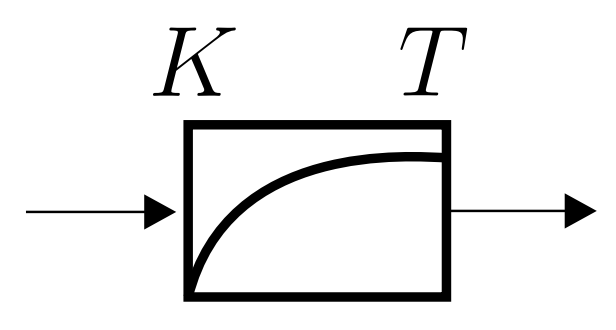
\includegraphics[width = \ImageWidth]{img/DIN-Symbole/PT1-Glied.png}}
           &
          $K (1-e^{-\frac{t}{T}})$
           &
          \raisebox{-.5\height}{
                \resizebox{\ImageWidth}{!}{%
                      \begin{tikzpicture}
                            % Grid
                            \draw[help lines,dashed] (0,0) grid (5,3);

                            % Axes
                            \draw[very thick,latex-latex] (0,3.25) node[left]{$y(t)$}
                            |- (5.25,0) node[below]{$t$};

                            % Plot function
                            \draw[ultra thick,teal] (-0.5,0) node[left,black](s0){$0$}
                            -- ++(0.5,0)
                            plot[domain=0:5,
                                        samples = 50,
                                        smooth]({\x},{2.5*(1- exp(-(\x)))});
                      \end{tikzpicture}
                }
          }
          \\
          \hline
          %%%%%%%%%%%%%%%%%%%%%%%%%%%%%%%%%%%%%%%%%%%%%%%%%%%%%%%%%%%%%%%%%%%%%%%%%%%%%%%%%%%%%%%%%%%%%
          \textbf{PT\textsubscript{2}-Glied}
          {\tiny
                \newline K: Verstärkung
                \newline T: Zeitkonstante
                \newline $\zeta$: Dämpfungskonstante
          }
           &
          $T^2 \cdot \ddot{y}(t) + 2 \zeta T \cdot \dot{y}(t) + y(t) = K \cdot u(t)$
          \newline $y(t) = K \cdot x(t) + T^2 \cdot (-\ddot{y}(t)) - 2 \zeta T \cdot \dot{y}(t)$
          {\tiny
                      \newline $\zeta = \frac{h}{\sqrt{h^2 + \pi^2}}$
                      \newline $h = \log(\frac{y_m}{y_{\infty}})$
                }
           &
          $\frac{K}{T^2 + s^2 + 2 \zeta T s + 1}$
           &
          \raisebox{-.5\height}{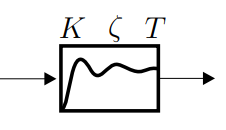
\includegraphics[width = \ImageWidth]{img/DIN-Symbole/PT2-Glied.png}}
           &
          $KA(1+e^{\sigma t}(-cos(\omega t) + \frac{\sigma}{\omega}sin(\omega t)))$
          {\tiny
                      \newline $\omega = \frac{2\pi}{T_m}$
                      \newline $K = \frac{y_{\infty}}{A} $
                      \newline $\sigma = \frac{h\omega}{\pi}$
                }
           &
          \raisebox{-.5\height}{
                \resizebox{\ImageWidth}{!}{%
                      \begin{tikzpicture}
                            % Grid
                            \draw[help lines,dashed] (0,0) grid (5,3);

                            % Axes
                            \draw[very thick,latex-latex] (0,3.25) node[left]{$y(t)$}
                            |- (5.25,0) node[below]{$t$};

                            % Plot function
                            \draw[ultra thick,teal] (-0.5,0) node[left,black](s0){$0$}
                            -- ++(0.5,0)
                            plot[domain=0:5,
                                        samples = 100,
                                        smooth]({\x},{1-exp(-0.3*3*\x)*(cos(deg(sqrt(1-0.3^2)*3*\x))+0.3/(sqrt(1-0.3^2))*sin(deg(sqrt(1-0.3^2)*3*\x)))
                                        });
                      \end{tikzpicture}
                }
          }
          \\
          \hline       
    \end{tabularx}
    \tiny{
          \\
          1. UTF = Übertragungsfunktion (Laplacetransformierte Sprungantwort)\\
          2. Proportionalglied ist einziges Statisches glied.\\
    }
    \endgroup
    \normalsize
\end{landscape}


\section{\tiltewithref{Klassifizierung von Systemen}{76,78,81}}
\begin{tabular}{|p{10cm}|p{10cm}|}
      \hline
      \rowcolor{TabularTitleColor}
      \textbf{Statisch} & \textbf{Dynamisch} \\
      \begin{itemize}   
            \item System ohne Gedächtnis
            \item Ausgang hängt nur von aktuellem Eingang ab.
            \item $y(t) = f(x(t)) \forall t$
      \end{itemize}
      & 
      \begin{itemize}     
            \item System mit Gedächtnis
            \item Ausgang hängt von aktuellem sowie vergangenen und zukünftigen Eingängen ab.
            \item $y(t) = f(x(t \pm t_0)) $ 
      \end{itemize}
      \\
      \hline
      \rowcolor{TabularTitleColor}
      \textbf{Kausal} & \textbf{Akausal} \\
      \begin{itemize}
            \item Ausgang \textbf{unabhängig} von zukünftigen Werten
            \item $y(t) = f(x(t-t_0)) $
      \end{itemize}
      &
      \begin{itemize}
            \item Ausgang \textbf{abhängig} von zukünftigem Eingang
            \item $y(t) = f(x(t+t_0)) $
      \end{itemize}
      \\
      \hline
      \rowcolor{TabularTitleColor}
      \textbf{Linear} & \textbf{Nicht-Linear}\\
      \begin{itemize}
            \item Linearkombination am Eingang -> Linearkombination am Ausgang
            \item Lineare DGL mit konstanten Koeffizenten
            \item $\Phi(\alpha x_a(t)+\beta x_b(t)) =\alpha y_a(t) + \beta y_b(t)$
            \item $\Phi(0) = 0$
      \end{itemize}
      & 
      \begin{itemize}
            \item Ausgang ist nicht immer Proportional zum Eingang 
            \item Keine Superposition
            \item Neue Frequenzanteile werden erzeugt
      \end{itemize}

      \\
      \rowcolor{TabularTitleColor}
      \textbf{Zeitinvariant} & \textbf{Zeitvariant}\\
      \begin{itemize}
            \item Zeitliche Verschiebung am Eingang -> gleiche Zeitliche Verschiebung am Ausgang
            \item $\Phi(x(t-t_v)) = y(t-t_v)$
      \end{itemize} 
      &
      \begin{itemize}
            \item Zeitinvarianz ist nicht erfüllt
            \item y(t) enthält t unabhägig von x(t)
      \end{itemize} 
      \\
      \hline
  
\end{tabular}


\newpage
%%%%%%%%%%%%%%%%%%%%%%%%%%%%%%%%%%%%%%%%%%%%%%
%Includes + Defines
%%%%%%%%%%%%%%%%%%%%%%%%%%%%%%%%%%%%%%%%%%%%%%

%\usepackage{color, colortbl}
%\usepackage{trfsigns}
%\usepackage{graphicx}
%\definecolor{TabularBackgroundColor}{rgb}{0.83,0.96,0.96}
%\usepackage{mathrsfs}


%%%%%%%%%%%%%%%%%%%%%%%%%%%%%%%%%%%%%%%%%%%%%%
%Content
%%%%%%%%%%%%%%%%%%%%%%%%%%%%%%%%%%%%%%%%%%%%%%
\section{Integraltransformationen}

\subsection{Faltung}
\begin{multicols}{2}

  $$y(t) = (x_1 * x_2)(t) = \int \limits _{-\infty} ^{\infty} x_1(\tau) \cdot x_2(t-\tau) d\tau$$
  \textbf{Eigenschaften:} \\
  \begin{tabular}{cc}
    Kommutativ  & ($f * g = g * f$)         \\
    Assoziatiov & ($(f*(g*h)) = ((f*g)*h)$) \\
    Distributiv & ($f*(g+h)= f*g + f*h$)    \\
    Stetigkeit  & ist \textbf{immer} stetig
  \end{tabular}

  \subsubsection*{Vorgehen}
  \begin{enumerate}
    \item $\tau$ bzw. $t-\tau$ in die Entsprechende Funktion Einsetzen
    \item Bereiche Bestimmen an denen die Funktion $\neq 0$
    \item Bereiche bzw. eingesetzte Funktionen in Hilfsdiagramm einzechnen (siehe Bsp.)
    \item Einzelne Integrationsbereiche mit Hilfe Diagramm bestimmen,
          indem Zeit $t$ "raufgezählt" und übergänge der Grenzen beachtet wird
    \item Integrale Bestimmen, Integralgrenzen = Eingezeichnete Grenzen im Diagramm.
    \item Integrale auflösen
  \end{enumerate}
  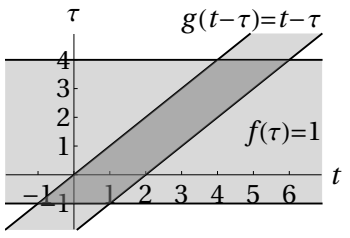
\includegraphics[width = 4.5cm]{include/Integraltransformationen/img/Faltungsgrenzen.png}
  \\\textbf{Beispiel}
  \\$f(t)= \begin{cases}
    2 \textrm{ für } 0 <t<4 \\
    0 \textrm{ sonst}
  \end{cases}
  g(t) = \begin{cases}
    3 \textrm{ für } 0<t<1 \\
    0 \textrm{ sonst}
  \end{cases}$
    \\1.$(f * g)(t) \int \limits _{-\infty} ^{\infty} f(\tau)g(t-\tau)d\tau$
    \\2.  $f(t): 0<\tau<4g(t): 0<t-\tau<1 \Rightarrow t-1 < \tau < t$
    \\3.  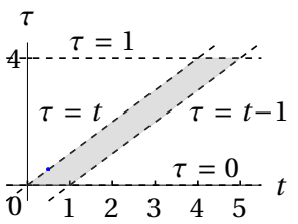
\includegraphics[width = 2cm]{include/Integraltransformationen/img/Bsp_Grenzen.png}
    \\4. und 5. $(f*g)(t) =$
    \\$t \leq 0: 0$
  \\$0 < t \leq 1: \int \limits _0 ^t 2 \cdot 3 d\tau$
    \\$1<t \leq 4: \int \limits _{t-1} ^t 2\cdot 3 d\tau$
  \\$4 <t \leq 5: \int \limits _{t-1} ^4 2\cdot 3 d\tau$
    \\$5< t: 0$

\end{multicols}


\subsection{Fourier-Reihe und Transformation}
\subsubsection*{Fourier-Reihe}
\begin{tabular}{p{4.5cm}p{11.5cm}}
  Trigonometrische Form    &
  $x(t) = \frac{a_0}{2} + \sum \limits _{n = 1} ^{\infty} a_n \cdot cos(2\pi n f_0 \cdot t) + b_n \cdot sin(2\pi n f_0 \cdot t) $
  \newline $a_n = \frac{2}{T} \int \limits _{T} x(t) dt$
  \newline $a_n = \frac{2}{T} \int \limits _{T} x(t) \cdot cos(2\pi n f_0 \cdot t)dt$
  \newline $b_n = \frac{2}{T} \int \limits _{T} x(t) \cdot sin(2\pi n f_0 \cdot t)dt$
  \\
  \rowcolor{TabularBackgroundColor}
  Harmonische Form         &
  $x(t) = r_0 + \sum \limits _{n = 1} ^{\infty} r_n \cdot cos(2\pi n f_0 \cdot t + \varpi_n)$
  \newline $r_0 = \frac{u_0}{2} = \frac{1}{T} \int  \limits _{T} x(t) dt $
  $r_n > 0 = \sqrt{u_n^2 + v_n^2}$
  $\varphi = arg(u_n - j \cdot v_n) $
  \\
  Komplexe Form            &
  $x(t) = \sum \limits _{n= -\infty} ^{\infty} c_n \cdot e^{jn2\pi f_0 \cdot t}$
  \newline $c_n =\overline{c_{-n}} = \frac{1}{T} \int \limits _{0} ^{T} x(t) \cdot e^{-j n 2 \pi f_0 \cdot t} dt$
  \newline $ 2\pi f_0$ wird auch als \textbf{Kreisfrequenz}  $\omega$ bezeichnet, \newline $f_0$ = Frequenz des Grundsignals $x(t)$.
  \\
  \rowcolor{TabularBackgroundColor}
  Umrechnung Koeffizienten &
  $c_n =\overline{c_{-n}} = \frac{a_n - jb_n}{2} (n = 0,1,2,3,..., b_0 =0)$
  \newline $a_n = 2 \cdot Re(c_n); \; b_n = -2 \cdot Im(c_n) (n = 0,1,2,3,..., b_0 =0)$ \\
\end{tabular}

\begin{multicols}{2}

  \subsubsection*{Fouriertransformation $\mathcal{F}(\omega)$}
  $$ X(\omega) = \mathcal{F}[x(t)] = \int \limits _{-\infty} ^{+\infty} x(t) \cdot e^{-j \omega t} dt $$
  $$ x(t) = \mathcal{F}^{-1}[X(\omega)] = \frac{1}{2 \pi} \int \limits _{- \infty} ^{+ \infty} X(\omega) \cdot e^{j \omega t} d\omega$$
  Rechenregeln Siehe Anhang.


  \subsubsection*{Spektraldarstellung}
  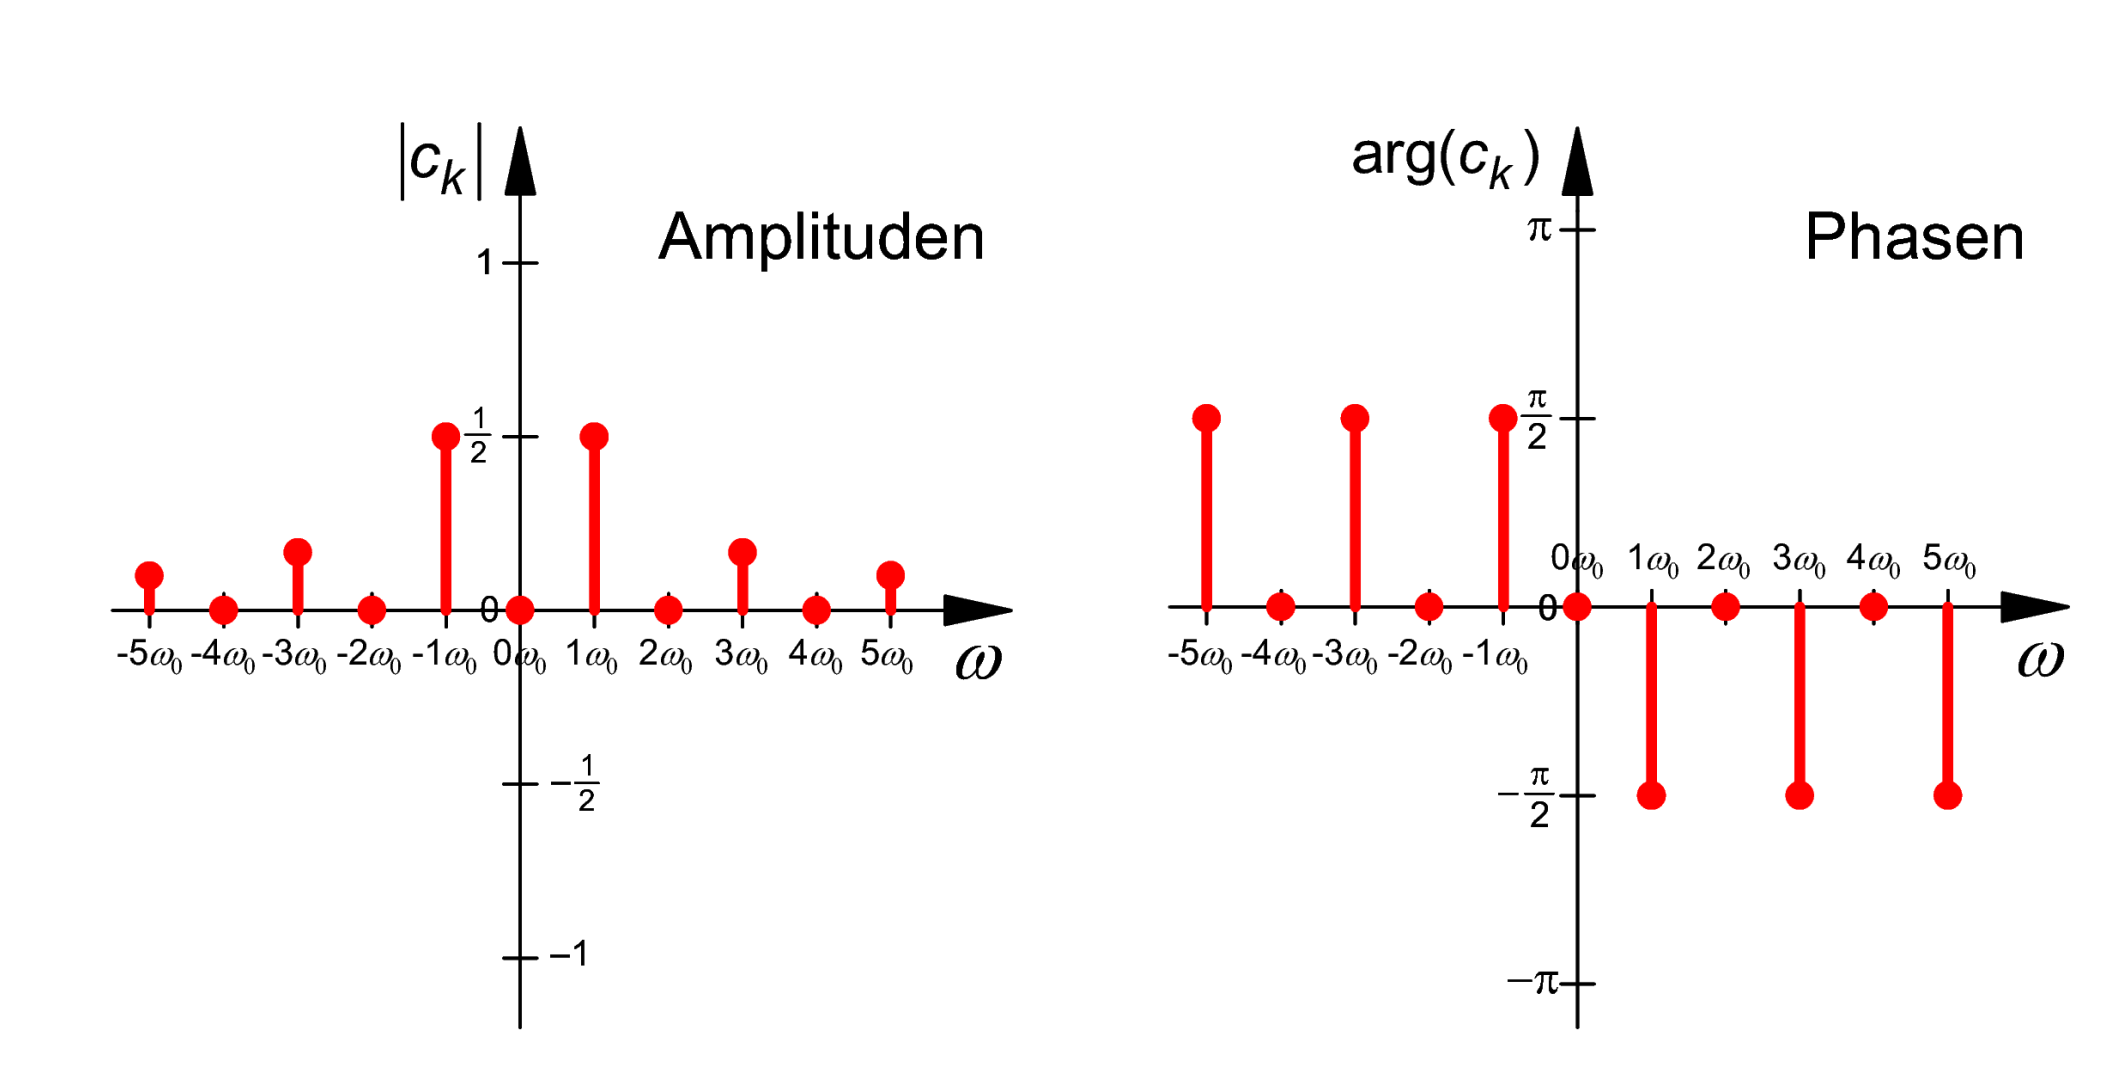
\includegraphics[width = 6cm]{include/Integraltransformationen/img/Spektrum.png}
\end{multicols}

\subsection{Laplace-Transformation}
\begin{multicols}{2}

  $$F(s) = \mathscr{L} {f(t)} = \int \limits _{0} ^{\infty} f(t) \cdot e^{-st} dt \textrm{ mit } s \in \mathbb{C}$$
  $$f(t) = \mathscr{L}^{-1} {f(t)} = \frac{1}{2\pi j} \int \limits _{p_0-j\infty} ^{p_0 + j\infty} F(s) \cdot e^{st} ds$$
  Rechenregeln Siehe Anhang.
  \subsubsection*{Lineare Differenzialgleichungen lösen:}
  DGL in Bildbereich Transformieren \\ $\Rightarrow$ DGL ist jetzt lineare Gleichung
  \\Gleichung auflösen
  \\Lösung Rücktransformieren

  \subsubsection*{Zusammenhänge}
  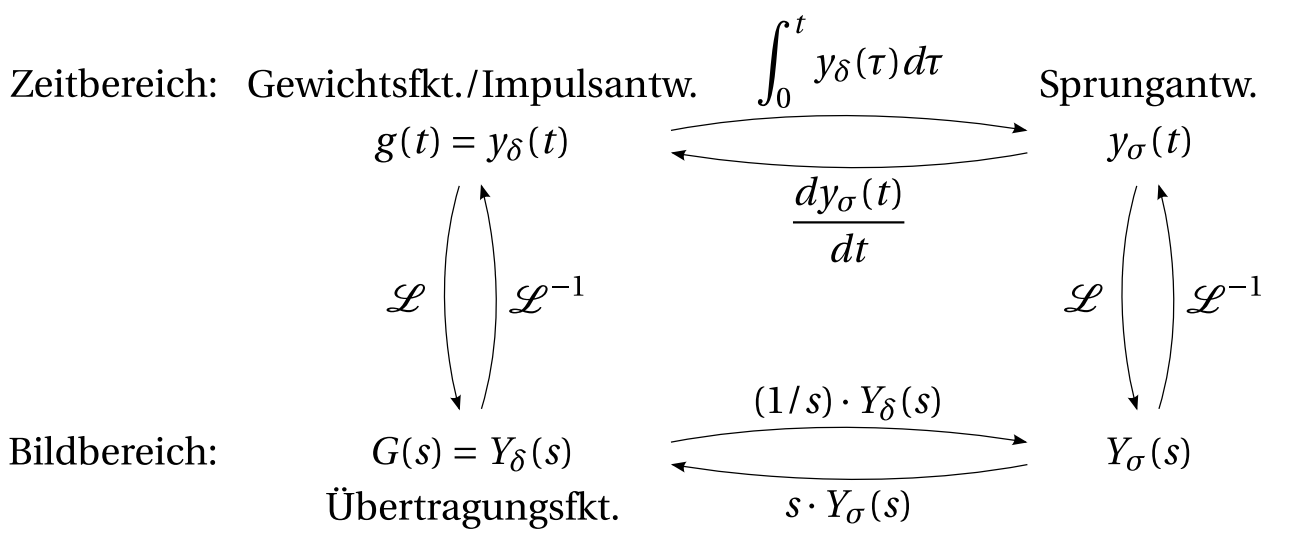
\includegraphics[width = 7cm]{include/Integraltransformationen/img/Zusammenhang_Laplace.png}

  \subsubsection*{Konvergenzhalbebene}
  Die Konvergenzhalbebene beginnt bei der Polstelle der Laplace-Transformierten mit dem Grössete Realteil und geht bis unendlich.
  \newline Bsp: Bei $\frac{1}{s-2}$ ist die Polstelle bei $+2$, daraus folgt: Konvergenzhalbebene $= [2,\infty)$
\end{multicols}

\subsection{Hilbert-Transformation}
\begin{multicols}{2}
  Im \textbf{Zeitbereich:}
  $$\hat{x}(t) = x(t) * \frac{1}{\pi t} = \frac{1}{\pi} \int \limits _{-\infty} ^{\infty} \frac{x(\tau)}{t-\tau} d\tau$$
  Im \textbf{Frequenzbereich}:
  $$\hat{X}(\omega) = X(\omega) \cdot H(\omega) = -j \cdot sgn(\omega) \cdot X(\omega)$$
\end{multicols}

%%%%%%%%%%%%%%%%%%%%%%%%%%%%%%%%%%%%%%%%%%%%%%
%Includes + Defines
%%%%%%%%%%%%%%%%%%%%%%%%%%%%%%%%%%%%%%%%%%%%%%

%\usepackage{color, colortbl}
%\usepackage{trfsigns}
%\usepackage{graphicx}
%\usepackage{adjustbox}
%\definecolor{TabularBackgroundColor}{rgb}{0.83,0.96,0.96}


%%%%%%%%%%%%%%%%%%%%%%%%%%%%%%%%%%%%%%%%%%%%%%
%Content
%%%%%%%%%%%%%%%%%%%%%%%%%%%%%%%%%%%%%%%%%%%%%%

\section{Wichtige Funktionen}

\small

\subsubsection*{Diracimpuls \tiny (auch Impuls-/Deltafunktion,-Distribution)}

\begin{multicols}{2}

  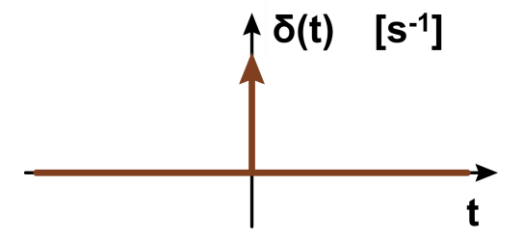
\includegraphics[width = 5cm]{include/Wichtige Funktionen/img/Impulsfunktion.png}

  {\footnotesize
    Unendlich kurzer, normierter Impuls mit unendlicher Amplitude. }

  \resizebox{0.5\textwidth}{!}{%
    \begin{tabular}{ccl}
      \hline \rowcolor{TabularBackgroundColor}
      1.  & $\delta(-t) = \delta(t) $                                                                                            & gerade Funktion                        \\
      \hline
      2.  & $\delta(-t+t_0) = \delta(t-t_0)$                                                                                     & symmetrisch                            \\
      \hline \rowcolor{TabularBackgroundColor}
      3.  & $\delta(at)= \frac{1}{|a|}\delta(t)$                                                                                 & Skalierung                             \\
      \hline
      4.  & $\delta(\frac{t-t_0}{a}) = |a| \cdot \delta(t-t_0)$                                                                  & Skalierung und Verschiebung            \\
      \hline \rowcolor{TabularBackgroundColor}
      5.  & $\delta(t-t_0)f(t) = f(t_0)\delta(t-t_0)$                                                                            & Abtastung                              \\
      \hline
      6.  & $\int \limits _{-\infty} ^{\infty} \delta(t-t_0)f(t)dt = f(t_0)$                                                     & Siebungseigenschaft                    \\
      \hline \rowcolor{TabularBackgroundColor}
      7.  & $\int \limits _{-\infty} ^{\infty}  A\cdot \delta(t)dt = A$                                                          & Spezialfall Siebungseigenschaft        \\
      \hline
      8.  & $\delta(t-t_0) * f(t) = f(t-t_0)$                                                                                    & Faltung                                \\
      \hline \rowcolor{TabularBackgroundColor}
      9.  & $\delta(t-t_1) * \delta(t-t_2) = \delta(t-t_1-t_2)$                                                                  & Faltung                                \\
      \hline
      10. & $\delta(t) = \frac{du(t)}{dt}$                                                                                       & Ableitung Einheitssprung               \\
      \hline \rowcolor{TabularBackgroundColor}
      11. & $ \delta(t) = \lim _{\omega \to \infty} \frac{sin(\omega t)}{\pi t} $                                                & Definition                             \\
      \hline
      12. & $ \delta(t) = \lim _{\epsilon \to \infty} \frac{\epsilon}{\pi(t^2 + \epsilon^2)} $                                   & Definition                             \\
      \hline \rowcolor{TabularBackgroundColor}
      13. & $\delta(t) = \lim _{\epsilon \to 0} \frac{e^{-t^2/\epsilon}}{\sqrt{(\pi \epsilon)}} $                                & Definition                             \\
      \hline
      14. & $t^n \frac{d^n \delta(t)}{dt^n} = (-1)^n n! \delta(t)$                                                               & Ableitung                              \\
      \hline \rowcolor{TabularBackgroundColor}
      15. & $f(t) * \frac{d\delta(t-t_0)}{dt} = \frac{df(t-t_0)}{dt}$                                                            & Faltung mit Ableitung                  \\
      \hline
      16. & $\frac{d\delta(t)}{dt} = \frac{\delta(t)}{-t} = \lim _{\epsilon \to 0} \frac{-2\epsilon t}{\pi(t^2 + \epsilon^2)^2}$ & 1. Ableitung $\delta(t)$ = ungerade F. \\
      \hline \rowcolor{TabularBackgroundColor}
      17. & $1$ \laplace $2\pi\delta(\omega)$                                                                                    & Fourier                                \\
      \hline
      18. & $\delta(t)$ \laplace $1(\omega)$                                                                                     & Fourier                                \\
    \end{tabular}}
\end{multicols}
  \begin{tabular}{|p{3.5cm}|p{3.5cm}|p{2cm}|p{3cm}|p{3.5cm}|}
    \hline

    \textbf{Name}
     &
    \textbf{Definition}
     &
    \laplace
     &
    \textbf{Formelzeichen}
     &
    \textbf{plot}
    \\
    \hline
    Sprungfunktion
    \newline (Heaviside)
     &
    $\begin{cases}
         0 \textrm{ für }  t<0,               \\
         [\frac{1}{2} \textrm{ für }  t = 0,] \\
         1 \textrm{ für }  t >0.
       \end{cases}$
    \newline \tiny(machmal: 1 für $t=0$)
     &
    $\frac{1}{j\omega} + \pi\delta(\omega)$
     &
    $u(t), \sigma(t), h(t)$
     &
    \raisebox{-.5\height}{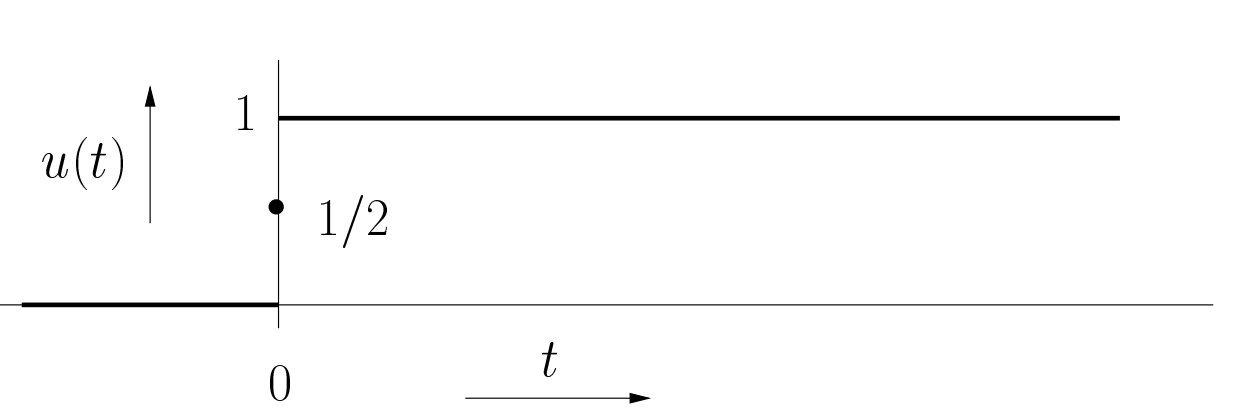
\includegraphics[width = 3.5cm]{include/Wichtige Funktionen/img/Sprungfunktion.png}}
    \\
    Signumfunktion
    \newline (Vorzeichenfunktion)
     &
    $\begin{cases}
         -1 \textrm{ für }  t<0,  \\
         0 \textrm{ für }  t = 0, \\
         1 \textrm{ für }  t >0.
       \end{cases}   $
     &
    $\frac{2}{j\omega}$
     &
    $sgn(t)$
     &
    \raisebox{-.5\height}{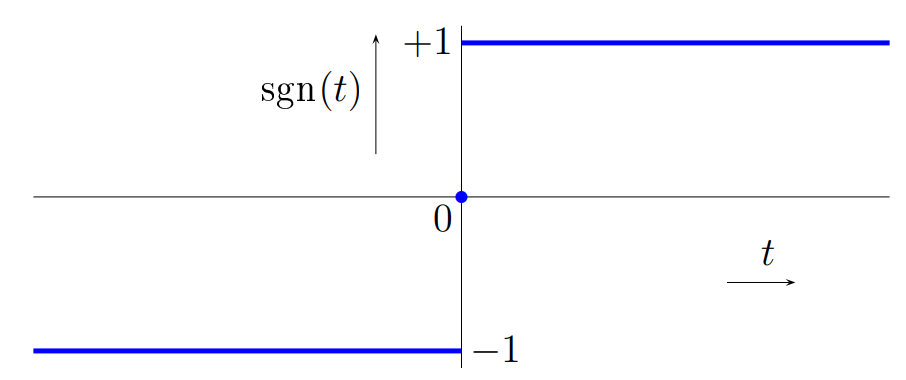
\includegraphics[width=3.5cm]{include/Wichtige Funktionen/img/Signumfunktion.png}}
    \\
    Rampenfunktion
     &
    $\begin{cases}
         0 \textrm{ für } t \leq 0, \\
         t \textrm{ für } t > 0.
       \end{cases}$
     &
    $\frac{1}{s^2}$
     &
    $r(t)$
     &
    \raisebox{-.5\height}{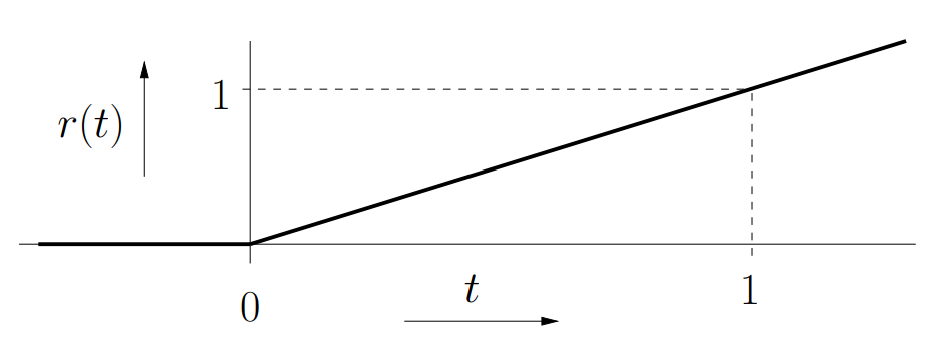
\includegraphics[width=3.5cm]{include/Wichtige Funktionen/img/Rampenfunktion.png}}
    \\
    Rechteckimpuls
     &
    $\begin{cases}
         1 \textrm{ für } |t| < a,           \\
         \frac{1}{2} \textrm{ für } |t| = a, \\
         0 \textrm{ für } |t| > a.
       \end{cases} $
     &
    $\frac{1}{s}- e^{-as}\frac{1}{s} $
     &
    $p_a(t), \beta(t)$
    \newline $\sigma(t+a)-\sigma(t-a)$
     &
    \raisebox{-.5\height}{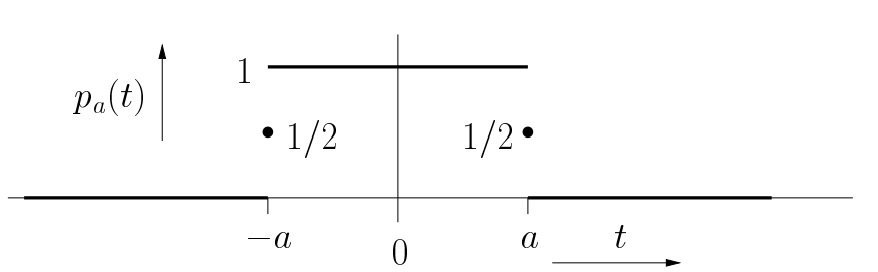
\includegraphics[width=3.5cm]{include/Wichtige Funktionen/img/Rechteckimpuls.png}}
    \\
    Dreieckimpuls
     &
    $\begin{cases}
         1 - \frac{|t|}{a} \textrm{ für } |t| < a \\
         0 \textrm{ für } |t| \geq a
       \end{cases}$
     &
    $sinc^2(\omega)$
     &
    $\Lambda(t)$
     &
    \raisebox{-.5\height}{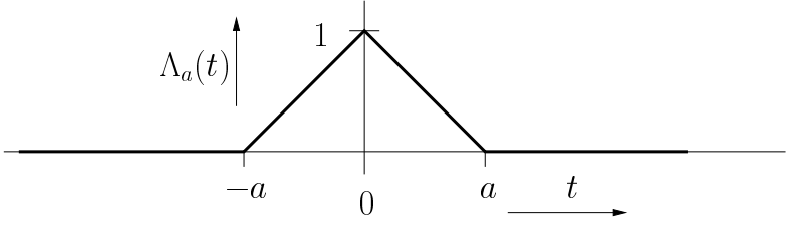
\includegraphics[width=3.5cm]{include/Wichtige Funktionen/img/Dreieckimpuls.png}}
    \\
    Sinc-Funktion
     &
    $\frac{sin(t)}{t}\; \forall t$
    \newline {\tiny $\lim _{t \to 0} sinc(t) = 1$}
    \newline {\tiny wenn normalisiert: $t \to \pi t$}
     &
    $\beta(\omega)$
    \newline{\tiny(Rechteckimpuls)}
     &
    sinc(t)
     &
    \raisebox{-.5\height}{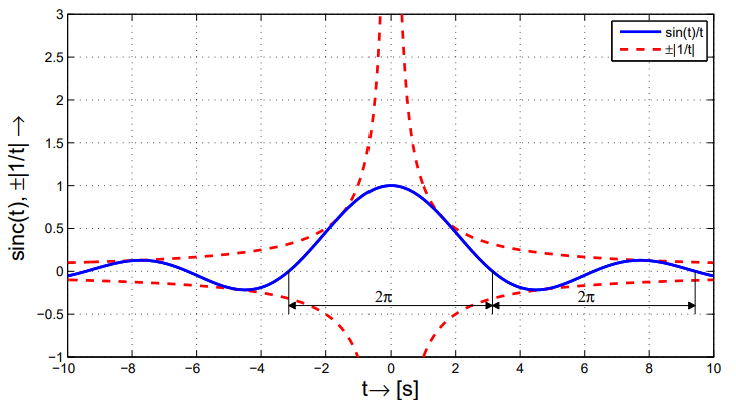
\includegraphics[width=3.5cm]{include/Wichtige Funktionen/img/SincFunktion.png}}
    \\
    \hline
  \end{tabular}
%Needs Package: 
%\usepackage{bm}
%\usepackage{multicol}
\section{LTI-Systeme}
\begin{minipage}{0.5\textwidth}

    \subsection*{Linearität und Zeitinvarianz}
    \begin{itemize}
        \item $\mathcal{T}[x_1(t) + x_2(t)] = y_1(t) + y_2(t)$
        \item $\mathcal{T}[k_a \cdot x(t)] = k_a \cdot y(t)$
        \item $\mathcal{T}[x(t-t_0) = y(t-t_0)]$
    \end{itemize}

    \subsection{Beschreibung von LTI Systemen}

    \subsubsection{Impulsantwort}
    Systemreaktion auf $\delta(t)$.

    $ y(t) = \mathcal{T}[x(t)]
        = \int \limits _{-\infty} ^{\infty} x(\tau) \cdot h(t-\tau)d\tau
        = x(t) * h(t)$

    \subsubsection{Frequenzantwort}
    Fouriertransformierte Impulsantwort.
    \\ Auch Übertragungsfunktion genannt.

    $$ Y(\omega) = X(\omega) \cdot H(\omega) = X(\omega) \cdot G(j\omega)$$

    \subsubsection{Berechnung des Ausgangssignals}
    1. Integraltransformation:
    \newline $X(\omega) = \mathcal{F}[x(t)] {\; \big / \;}
        X(s) = \mathscr{L}[x(t)]$ \\
    2. Berechnung in Bild / Frequenz:
    \newline $Y(\omega) = X(\omega) \cdot H(\omega)  {\; \big / \;}
        Y(s) = X(s) \cdot G(s)$ \\
    3. Rücktransformation:
    \newline $y(t) = \mathcal{F}^{-1}[Y(\omega)] = \mathscr{L}^{-1}[Y(s)]$

\end{minipage}%
\begin{minipage}{0.6\textwidth}


    \subsection{Bezeichnungen}
    Übertragungsfunktion: $H(\omega) = G(j\omega) =|H(\omega)| \cdot e^{j\varphi_H(\omega)}$ \\
    {\tiny auch: Frequenzgang}\\
    Amplitudengang: $|H(\omega)|$ \\
    Phasengang: $\varphi_H(\omega)$ \\

    \subsubsection{Filtereigenschaften}
    $Y(\omega) = X(\omega) \cdot H(\omega)$ \\
    $|Y(\omega)| = |X(\omega)| \cdot |H(\omega)|$ \\
    $\varphi_y(\omega) = \varphi_x(\omega) + \varphi_H(\varphi)$

    \subsection{BIBO-Stabilität \tiny {Bound-Input-Bound-Output}}

    Systemantwort Begrenzt, wenn Eingangssignal Begrenzt
    \newline $\Rightarrow$ Konvergenzhalbebene Übertragungsfunktion enthält Imaginär-Achse
    \newline $\Rightarrow$ Alle Polstellen Übertragungsfunktion links von "$j$-Achse"
    \begin{center}
        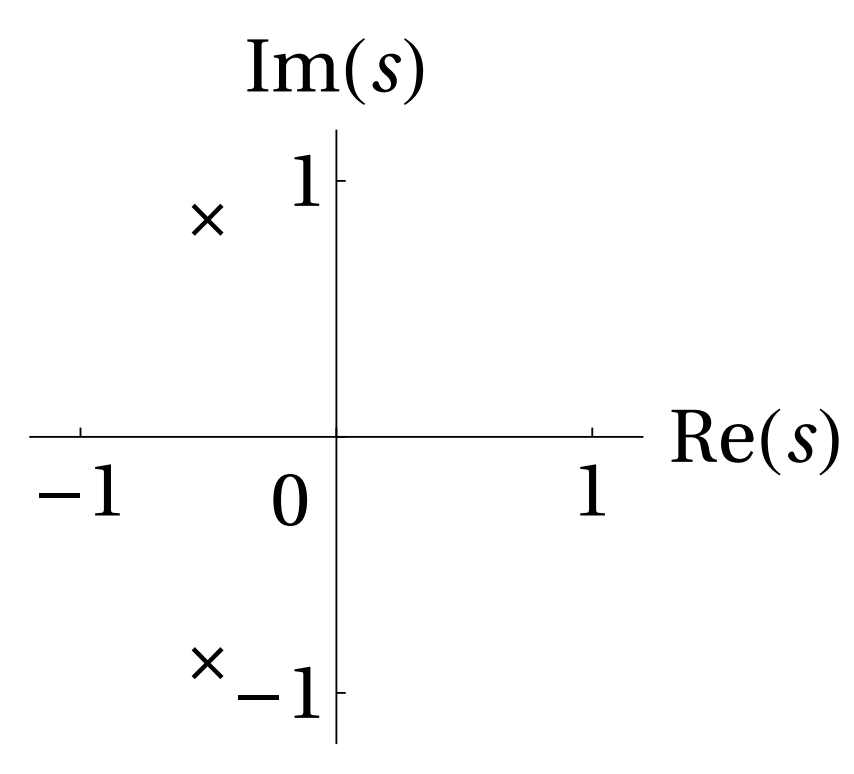
\includegraphics[width = 4cm]{include/Integraltransformationen/img/BiBo.png}
    \end{center}

\end{minipage}%

%%%%%%%%%%%%%%%%%%%%%%%%%%%%%%%%%%%%%%%%%%%%%%
%Includes + Defines
%%%%%%%%%%%%%%%%%%%%%%%%%%%%%%%%%%%%%%%%%%%%%%

%\usepackage{color, colortbl}
%\usepackage{trfsigns}
%\usepackage{graphicx}
%\definecolor{TabularBackgroundColor}{rgb}{0.83,0.96,0.96}


%%%%%%%%%%%%%%%%%%%%%%%%%%%%%%%%%%%%%%%%%%%%%%
%Content
%%%%%%%%%%%%%%%%%%%%%%%%%%%%%%%%%%%%%%%%%%%%%%


\section{Integrieren und Differenzieren}
\subsection{Integrationsregeln}
\begin{tabular}{ll}
  Linearit\"at                    & $\int{f(\alpha x+\beta )dx=\frac{1}{\alpha}\cdot F(\alpha x+\beta)+C}$ \\
  
  \rowcolor{TabularBackgroundColor}
  Partielle Integration           & $\int\limits_a^b{u'(x)\cdot v(x)dx}=\biggl[
      u(x)\cdot v(x) \biggr]_a^b-\int\limits_a^b{u(x)\cdot v'(x)dx}$
  \tiny($v(x)$ = einfacheste Funktion wählen!) \normalsize                                                 \\

  Substitution (Rationalisierung) & $t=\tan\frac{x}{2}, \qquad
    dx=\frac{2dt}{1+t^2} \qquad \sin  x=\frac{2t}{1+t^2} \qquad \cos x=\frac{1-t^2}{1+t^2}
  \quad\int{R(\sin(x)\cos(x))dx}$                                                                          \\
  
  \rowcolor{TabularBackgroundColor}
  Allgemeine Substitution         &
  $\int\limits_{a}^{b}{f(x)dx}=\int\limits_{g(a)}^{g(b)}{f(g(t))\cdot
  g'(t)dt}\qquad x=g(t)\qquad g'(t)=\frac{dt}{dx}\qquad dx=\frac{1}{g'(t)}\cdot dt$                        \\

  Logarithmische Integration      & $\int{\frac{f'(x)}{f(x)}dx}=\ln|f(x)|+C
  \qquad{(f(x)\neq 1)}$                                                                                    \\

  \rowcolor{TabularBackgroundColor}
  Spezielle Form des Integranden  & $\int{f'(x)\cdot
      (f(x))^{\alpha} dx}= f(x)^{\alpha +1}\cdot \frac{1}{\alpha+1}+C
  \qquad{(\alpha \neq -1)}$                                                                                \\

  Differentiation                 & $\int \limits ^{b} _{a} {f'(t)dt}=f(b)-f(a)$\qquad
  $\frac{d}{dx} \int \limits ^{x} _{1} {f(t)dt}=f(x)$
\end{tabular}
\\

\begin{minipage}{0.5\textwidth}
  \subsection{Ableitungsregeln}
  \begin{tabular}{ll}
    Linerität       & $(\lambda f + \mu g)'(x) = \lambda f'(x) + \mu g'(x)$ \\
    \rowcolor{TabularBackgroundColor}
    Produktregel    & $(f\cdot g)' = f'g + fg'$                             \\
    Quotientenregel & $(\frac{f}{g})' = \frac{f'g - fg'}{g^2}$              \\
    \rowcolor{TabularBackgroundColor}
    Kettenregel     & $ (f(g))' = f'(g) \cdot g' $                          \\
    Potenz          & $((x-a)^n)'= n\cdot(x-a)^{n-1}$                       \\
    \rowcolor{TabularBackgroundColor}
    Trigo           & $sin'' = cos' = -sin$                                 \\
    Schrittfunktion & $\sigma'(t) = \delta(t)$
  \end{tabular}
\end{minipage}%
\begin{minipage}{0.5\textwidth}
  \subsection{Partialbruchzerlegung}
  Nenner Faktorisieren (Nennerexponent)
  \\Zähler = Polynom (Nennergrad -1)
  \\Gleichsetzen mit Originalbruch
  \\Mit Gleichungssystem auflösen.
  \\Ansätze:
  \\ $\frac{\dots}{x(x-3)^2} = \frac{A}{x} + \frac{B}{x-3} + \frac{C}{(x-3)^2}$
  \\ $\frac{\dots}{(x-2)^3} = \frac{A}{x-2} + \frac{B}{(x-2)^2} + \frac{C}{(x-2)^3}$
  \\ $\frac{\dots}{x^4 + x^2} = \frac{A}{x} + \frac{B}{x^2} + \frac{Cx + D}{x^2 + 1}$
\end{minipage}
\section{Tabellen}

\subsubsection*{Blockschaltbilder MatLab}
\begin{tabular}{|c|c|c|c|c|}
      \hline
      \textbf{Summierer}                                            &
      \textbf{Differenzbilder}                                      &
      \textbf{Konstante}                                            &
      \textbf{Proportionalglied}                                    &
      \textbf{Integrierer}                                            \\
      
\includegraphics[]{img/matlab/sum_block_icon.png}             &
      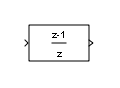
\includegraphics[]{img/matlab/difference_block_icon.png}      &
      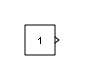
\includegraphics[]{img/matlab/constant_block_icon.png}        &
      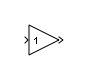
\includegraphics[]{img/matlab/gain_block_icon.png}            &
      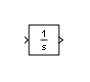
\includegraphics[]{img/matlab/integrator_block_icon.png}        \\
      \hline
      \textbf{Totzeitglied}                                         &
      \textbf{Differenzierer}                                       &
      \textbf{}                                                     &
      \textbf{}                                                     &
      \textbf{}                                                       \\
      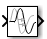
\includegraphics[]{img/matlab/transport_delay_block_icon.png} &
      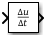
\includegraphics[]{img/matlab/derivative_block_icon.png}      &
      &
      &
      \\
      \hline
\end{tabular}

\end{document}
